Due to the imperfection simulation process, there will always be discrepancies between simulated samples and the actual collected data.
Methods of correction including event weights and alternation of kinematic values can be applied to ensure the physics are well matched to the data.

\subsection{Jet energy smearing}
The width of the jet kinematic, called the resolution, is wider in data than in simulation~\cite{CMS:2016lmd}.
The difference could be alleviated by scaling the reconstructed four momentum of simulated jets by some factor $c_{\mathrm{JER}}$, which is called the smearing.
The scaling method for obtaining $c_{\mathrm{JER}}$ can be given as
\begin{linenomath}\begin{equation}\label{eq:data_smear}
    c_{\mathrm{JER}} = 1 + (S_{\mathrm{JER}}-1)\biggl(\frac{\PT-\PT^{\mathrm{ptcl}}}{\PT}\biggr)
\end{equation}\end{linenomath}
where $(S_{\mathrm{JER}}$ represents the average ratio between the relative jet resolution measured in data and simulation and $\PT^{\mathrm{ptcl}}$ is the transverse momentum of the corresponding jet clustered from generator-level particles.
The factor $c_{\mathrm{JER}}$ is truncated at zero, i.e. if it is negative, it is set to zero. 
This method only works if a well-matched particle-level jet is present and a large shift in the jet energy might be applied otherwise.
The requirements of well-matched are defined as
\begin{linenomath}\begin{equation}\label{eq:data_wellmatched}
    \Delta R < \frac{R_{\mathrm{cone}}}{2};\; |\PT-\PT^{\mathrm{ptcl}}|<3\sigma_{\mathrm{JER}}\PT
\end{equation}\end{linenomath}
where $R_{\mathrm{cone}}$ is the jet cone size parameter and $\sigma_{\mathrm{JER}}$ is the relative \PT resolution as measured in simulation.
In the case of lacking well-matched generator level jet, a stochastic smearing should be use:
\begin{linenomath}\begin{equation}\label{eq:data_stochastic}
    c_{\mathrm{JER}} = 1 + N(0, \sigma_{\mathrm{JER}}) \sqrt{\mathrm{max}(S_{\mathrm{JER}}^2-1,0)}
\end{equation}\end{linenomath}
where $N(0,\sigma)$ denotes a random number sampled from a normal distribution with a zero mean and variance $\sigma^2$.
As before, this scaling factor $c_{\mathrm{JER}}$ is truncated at zero.

\subsection{Efficiency scale factor}
Scale factors are applied on a event-by-event basis to alleviate the discrepancies between data and simulation causing by different selection efficiency.
Take electron trigger for example, if the trigger efficiency turns out to be $\epsilon_{\mathrm{data}}$ while the simulated samples indicates the trigger efficiency to be $\epsilon_{\mathrm{sim}}$, a simulated event with one electron passing the trigger should be treated as $\epsilon_{\mathrm{data}}/\epsilon_{\mathrm{sim}}$ event.
Scale factors are typically derived in a $\eta-\PT$ plane to account for the geometry of the detector and different sensitivity of the reconstruction process at various energy scales.
Most of the efficiency scale factors used in this analysis are provided by their physics object group, except for the electron trigger and \PQb tagging algorithm.
The scale factors of electron trigger are studied independently and documented in Appendix~\ref{appendix:trigger}.
The event-by-event weight of \PQb tagging algorithm is obtained with the scale factors and MC \PQb tagging efficiencies defined as
\begin{linenomath}\begin{equation}\begin{aligned}\label{eq:data_btagsf}
    w &= \frac{P(\mathrm{Data})}{P(\mathrm{MC})}
\end{aligned}\end{equation}\end{linenomath}
with 
\begin{linenomath}\begin{equation}\begin{aligned}\label{eq:data_btageff}
    P(\mathrm{MC}) &= \prod_{\mathrm{i=tagged}} \epsilon_{i} \prod_{\mathrm{j=untagged}} (1-\epsilon_{j}) \\
    P(\mathrm{Data}) &= \prod_{\mathrm{i=tagged}} \mathrm{SF}_i\epsilon_{i} \prod_{\mathrm{j=untagged}} (1-\mathrm{SF}_j\epsilon_{j}) \\
\end{aligned}\end{equation}\end{linenomath}
where $w$ is the event weight, $\epsilon$ is the MC \PQb tagging efficiency, and SF is the scaling factor of \PQb tagging algorithm as a function of jet flavor, jet \PT, and jet $\eta$. 
The goal of this method is to predict the correct event yield in data by only changing the weight of the selected MC events, i.e., MC events that did not pass the selection do not need to be added back.
The efficiency of the \PQb tagging in different jet flavor are shown in Figs.~\ref{fig:reco_beff16},~\ref{fig:reco_beff17}, and~\ref{fig:reco_beff18}. 
\begin{figure}\centering
    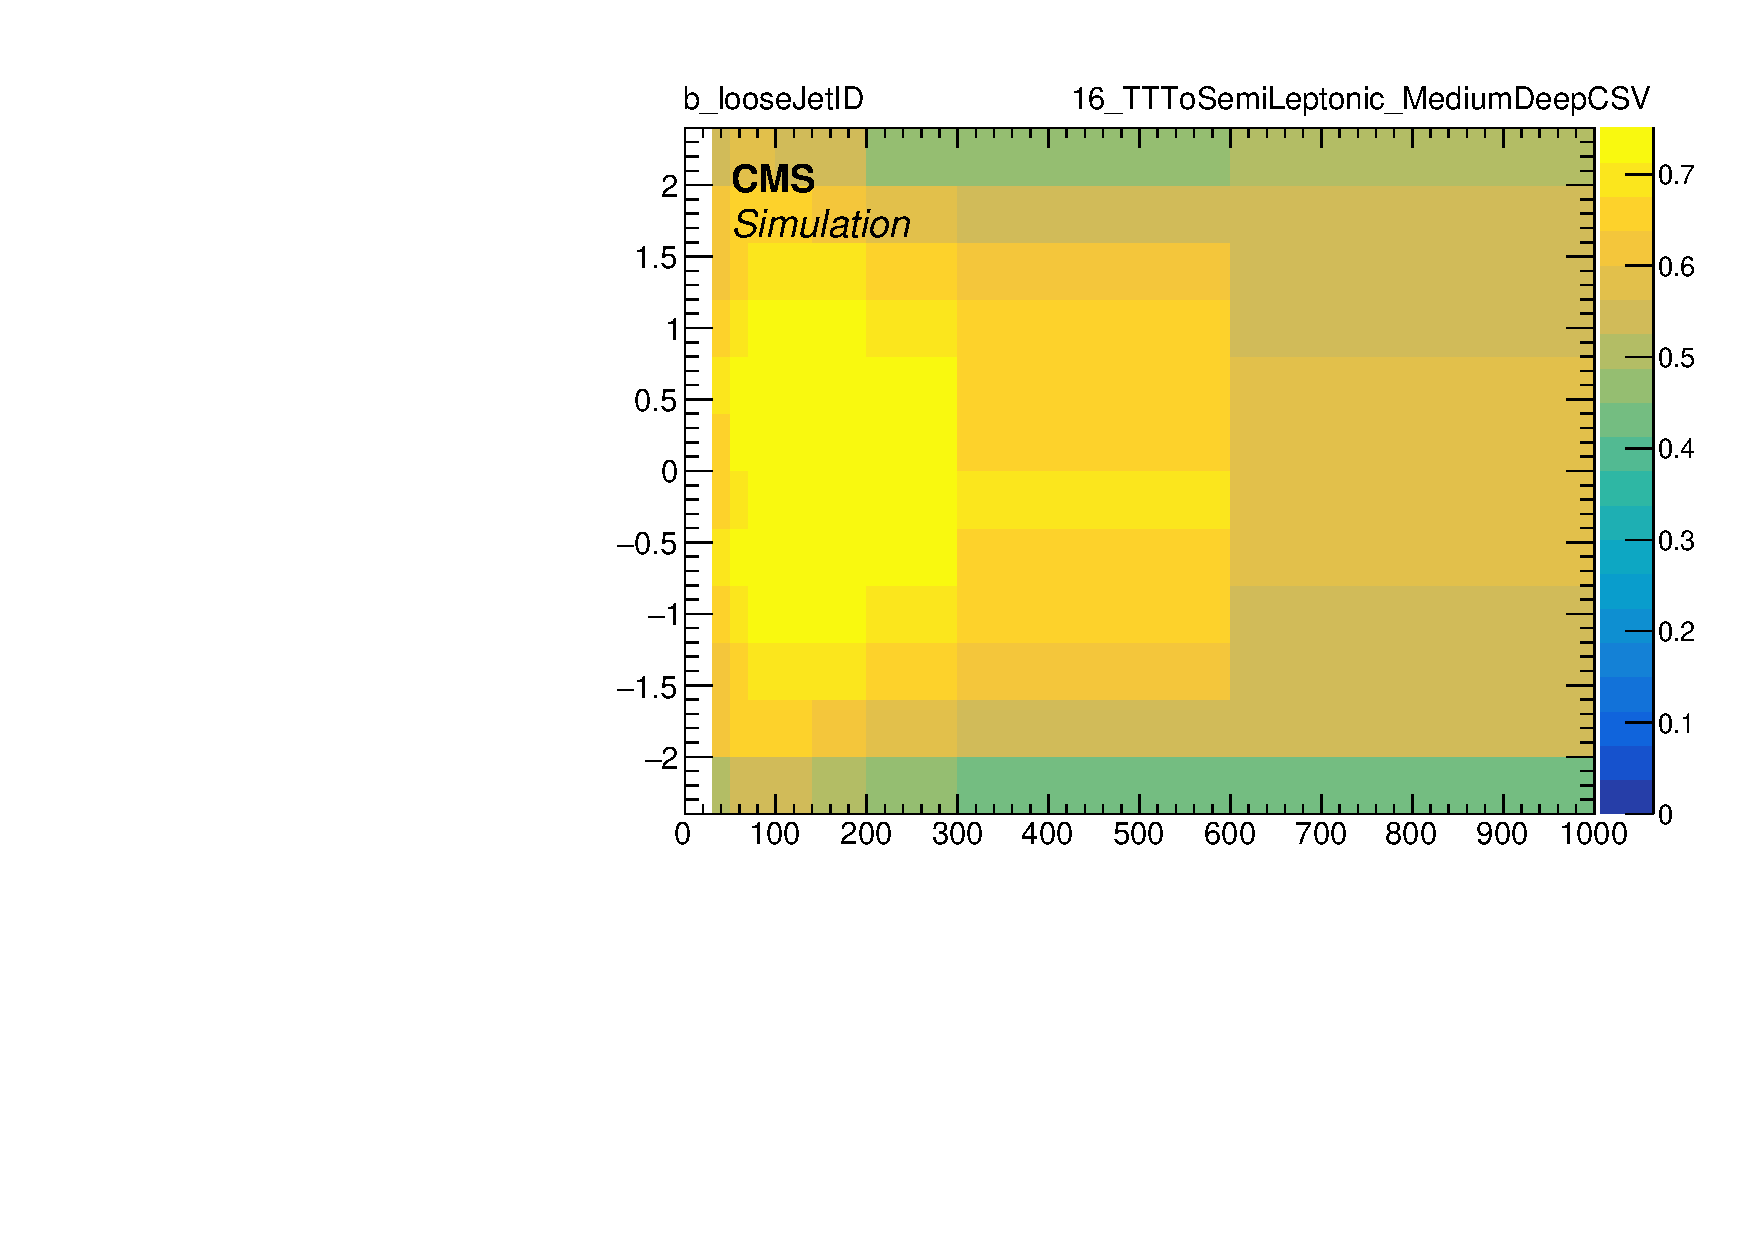
\includegraphics[width=0.4\textwidth]{figure/BtagEffPlot_16_TTToSemiLeptonic_eff2D_b_MediumDeepCSV.pdf}
    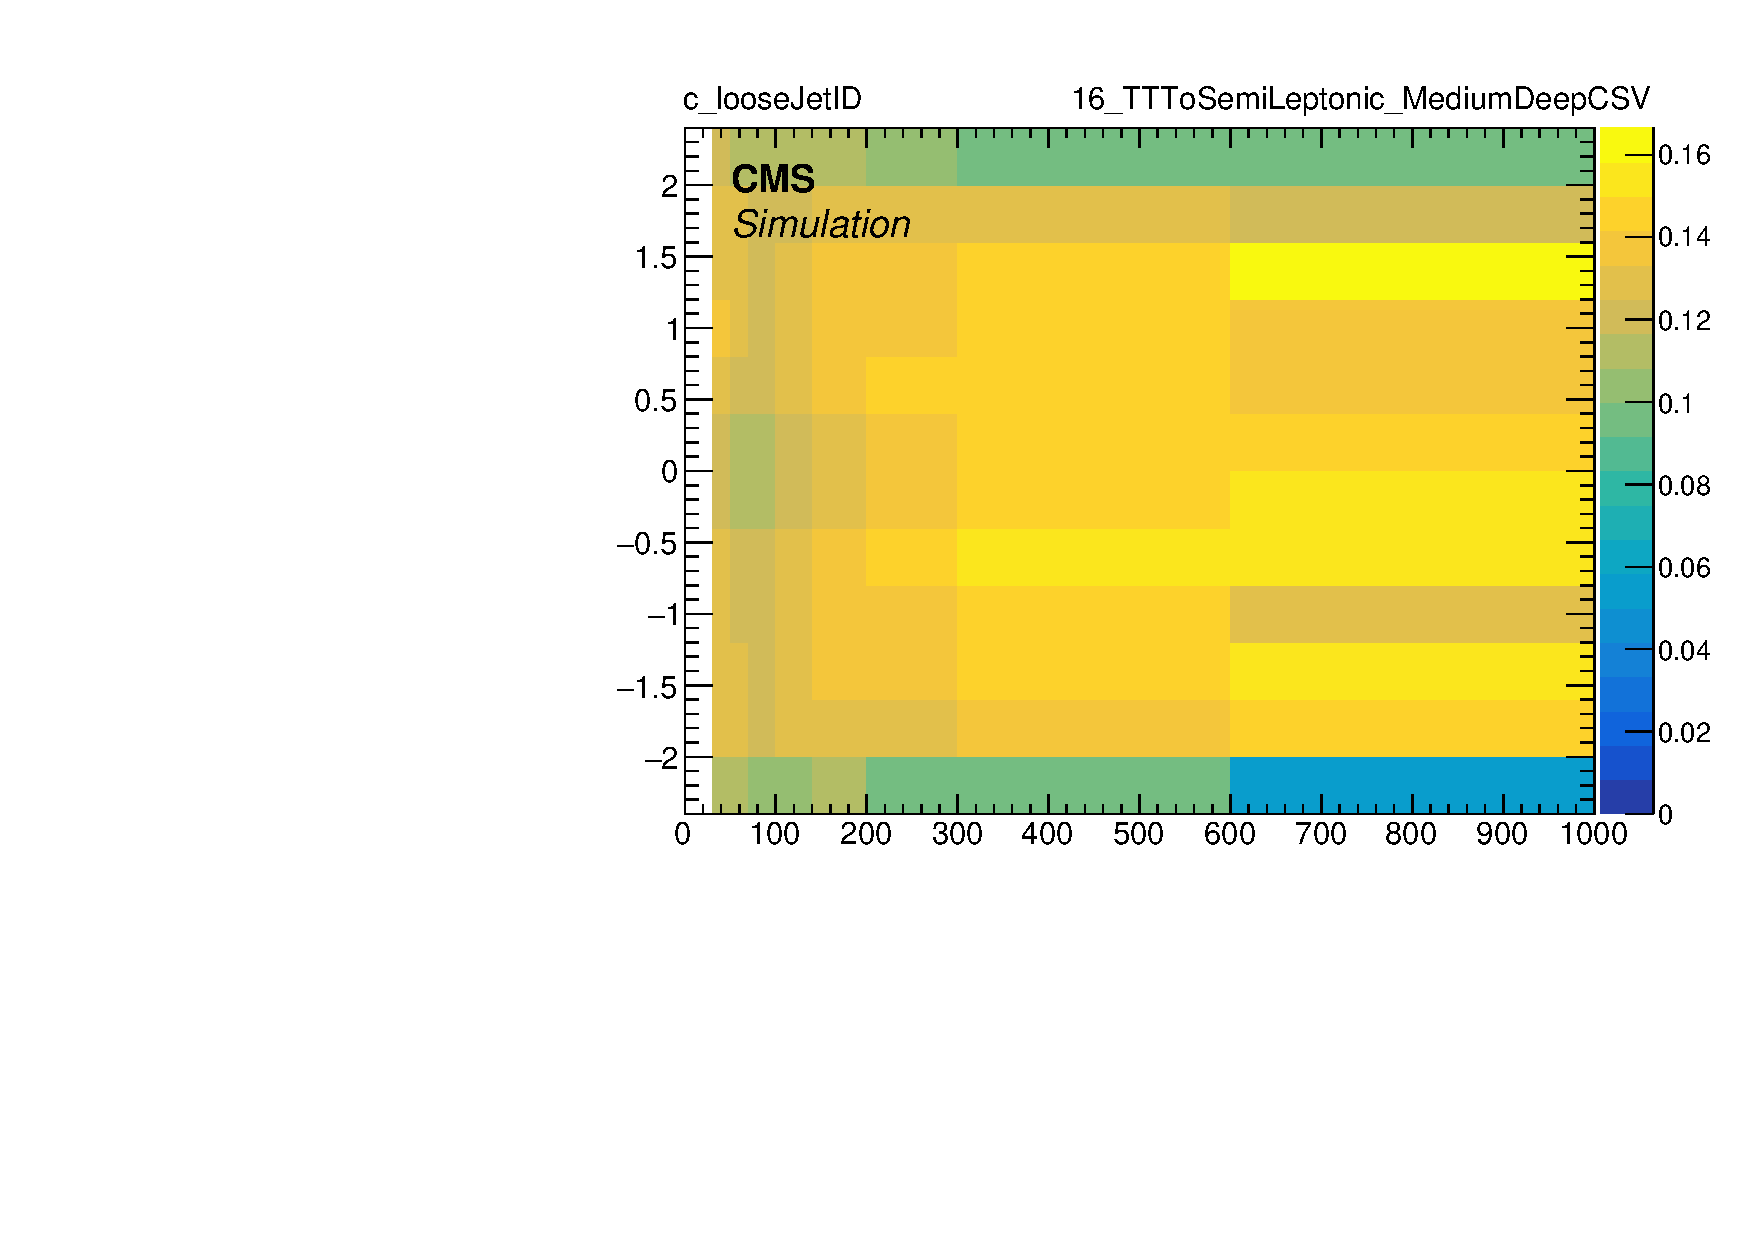
\includegraphics[width=0.4\textwidth]{figure/BtagEffPlot_16_TTToSemiLeptonic_eff2D_c_MediumDeepCSV.pdf}
    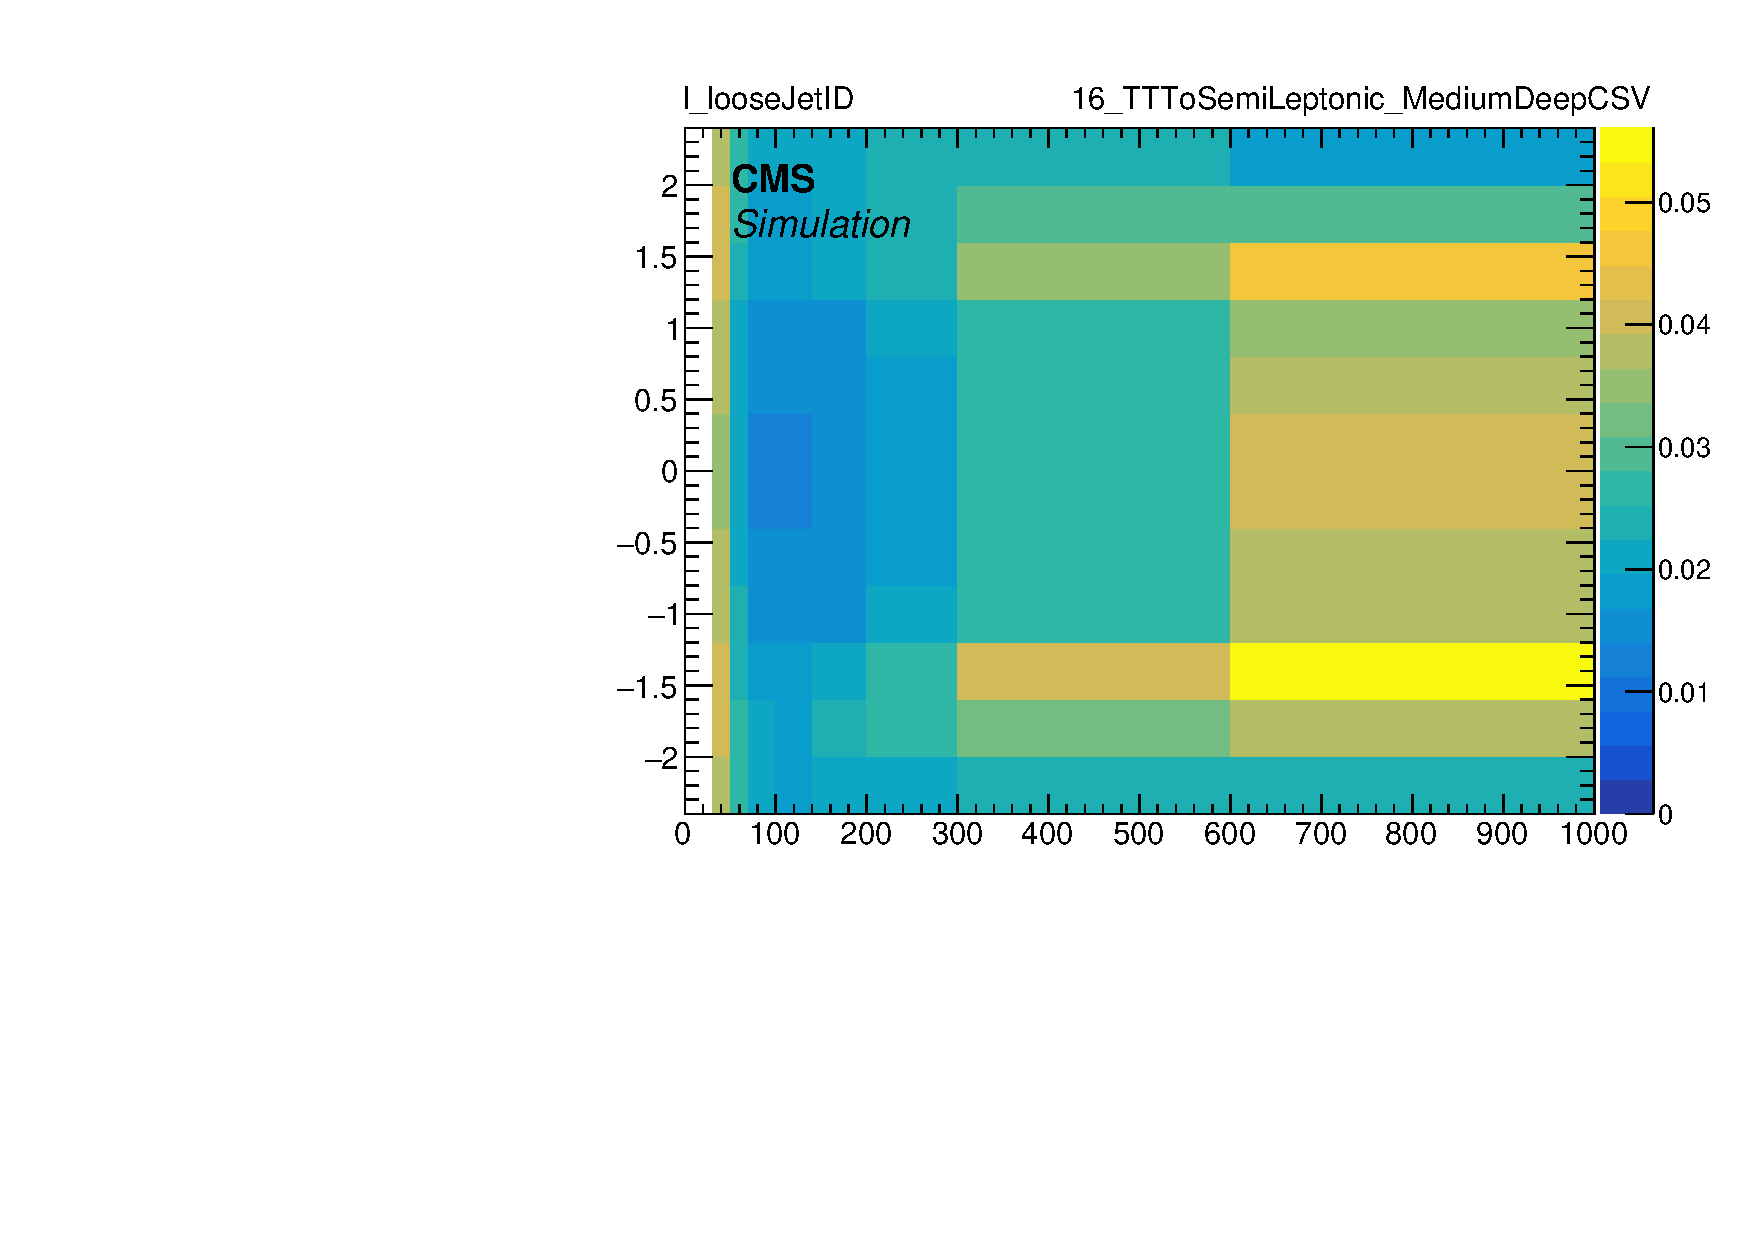
\includegraphics[width=0.4\textwidth]{figure/BtagEffPlot_16_TTToSemiLeptonic_eff2D_l_MediumDeepCSV.pdf}
    \caption[Display of \PQb tagging efficiency of 2016 \ttbar samples.]
    {
        Display of \PQb tagging efficiency of 2016 \ttbar samples for \PQb jet (left), \PQc jet (medium), and light jet (right) as functions of the jet \PT and jet $\eta$.
    }
    \label{fig:reco_beff16}
\end{figure}
\begin{figure}\centering
    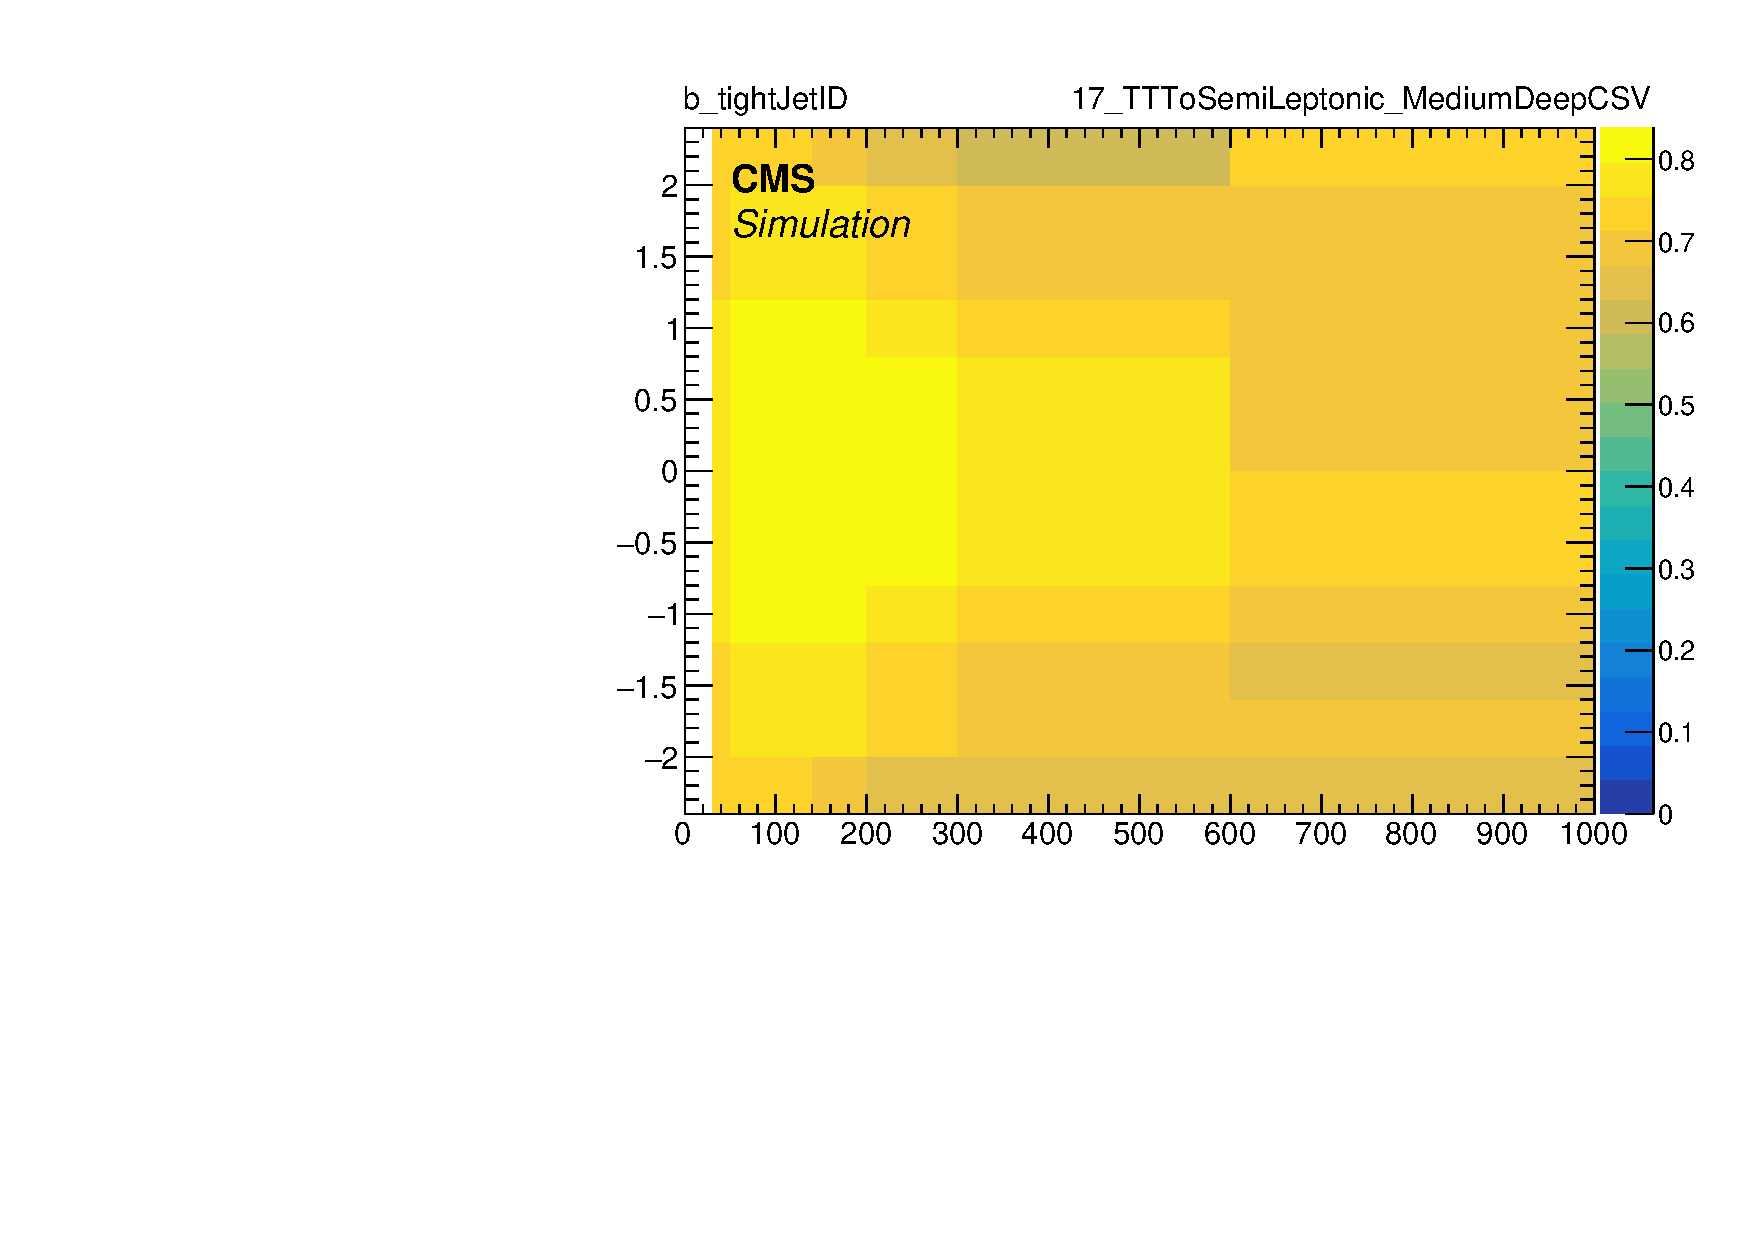
\includegraphics[width=0.4\textwidth]{figure/BtagEffPlot_17_TTToSemiLeptonic_eff2D_b_MediumDeepCSV.pdf}
    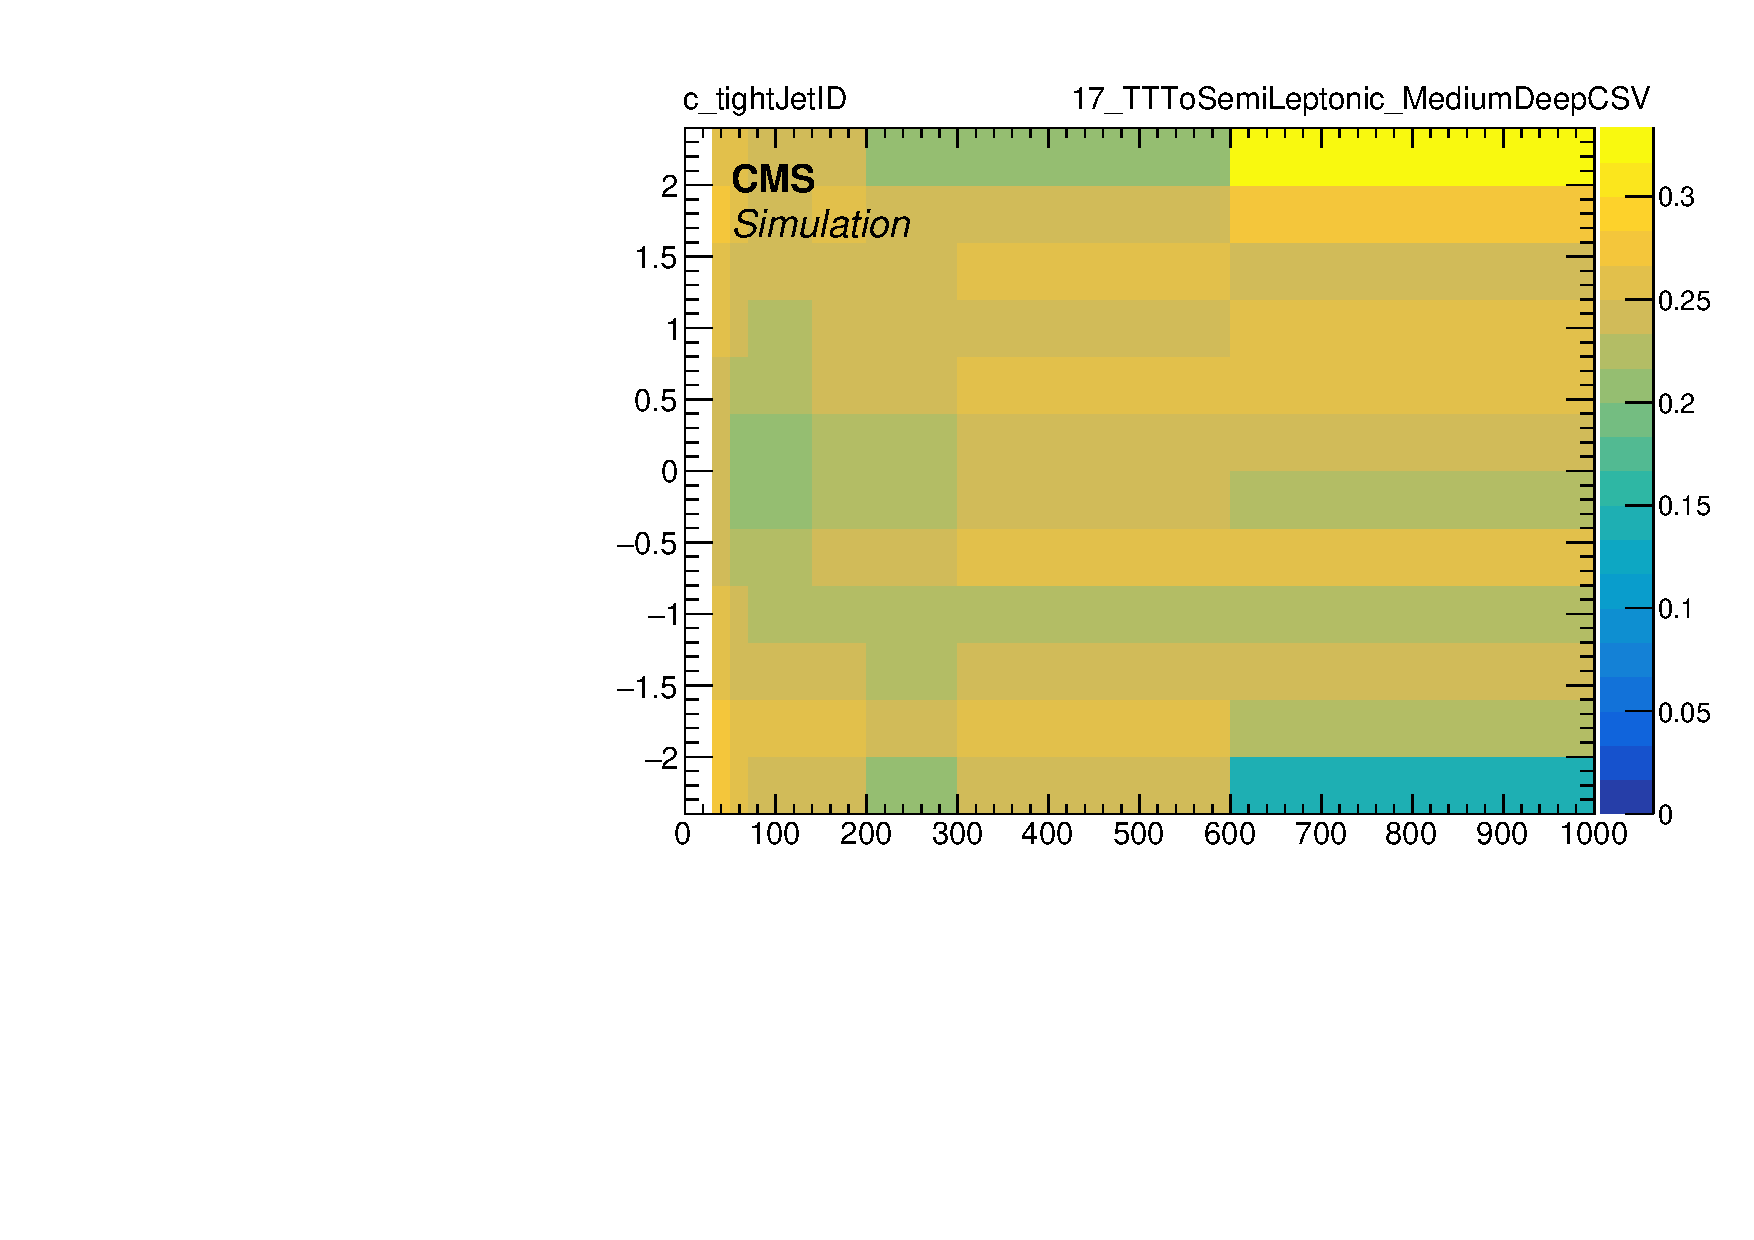
\includegraphics[width=0.4\textwidth]{figure/BtagEffPlot_17_TTToSemiLeptonic_eff2D_c_MediumDeepCSV.pdf}
    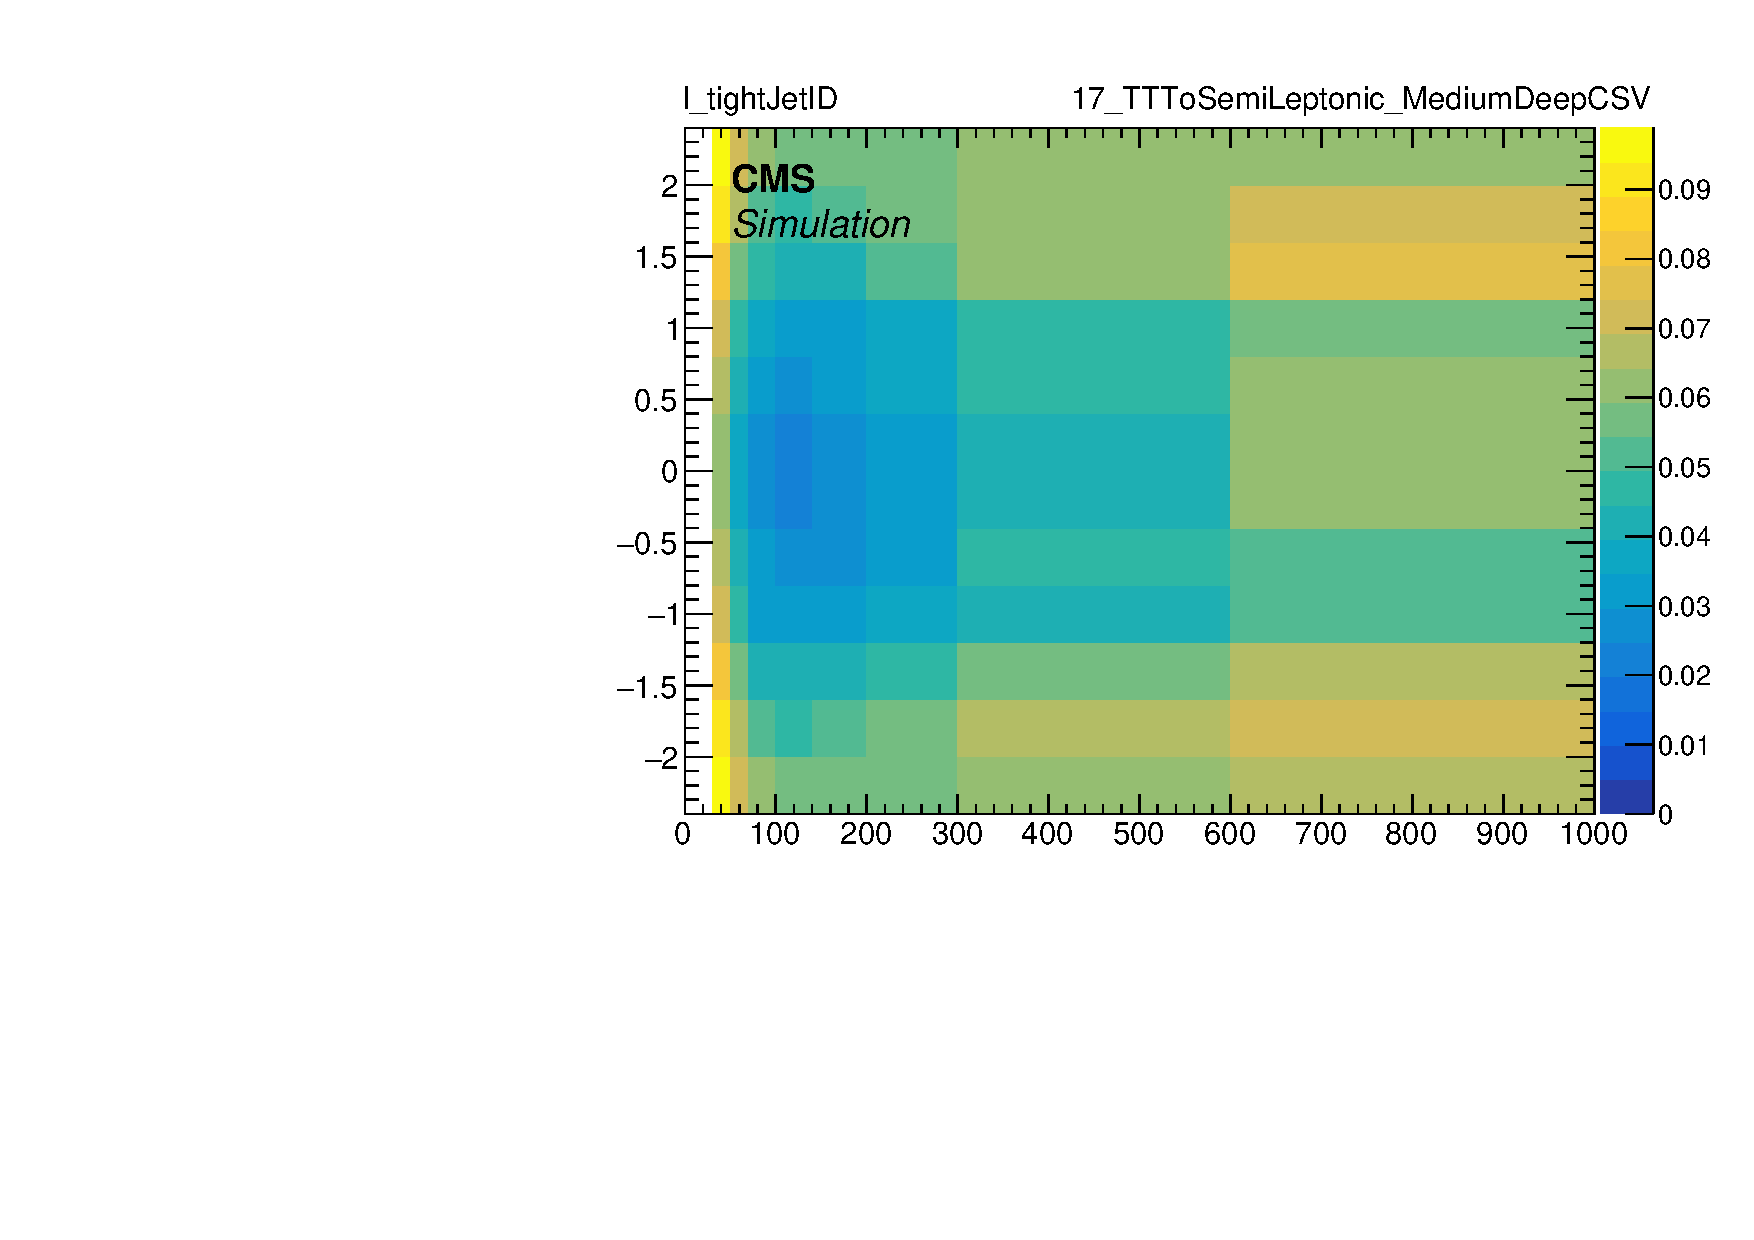
\includegraphics[width=0.4\textwidth]{figure/BtagEffPlot_17_TTToSemiLeptonic_eff2D_l_MediumDeepCSV.pdf}
    \caption[Display of \PQb tagging efficiency of 2017 \ttbar samples.]
    {
        Display of \PQb tagging efficiency of 2017 \ttbar samples for \PQb jet (left), \PQc jet (medium), and light jet (right) as functions of the jet \PT and jet $\eta$.
    }
    \label{fig:reco_beff17}
\end{figure}
\begin{figure}\centering
    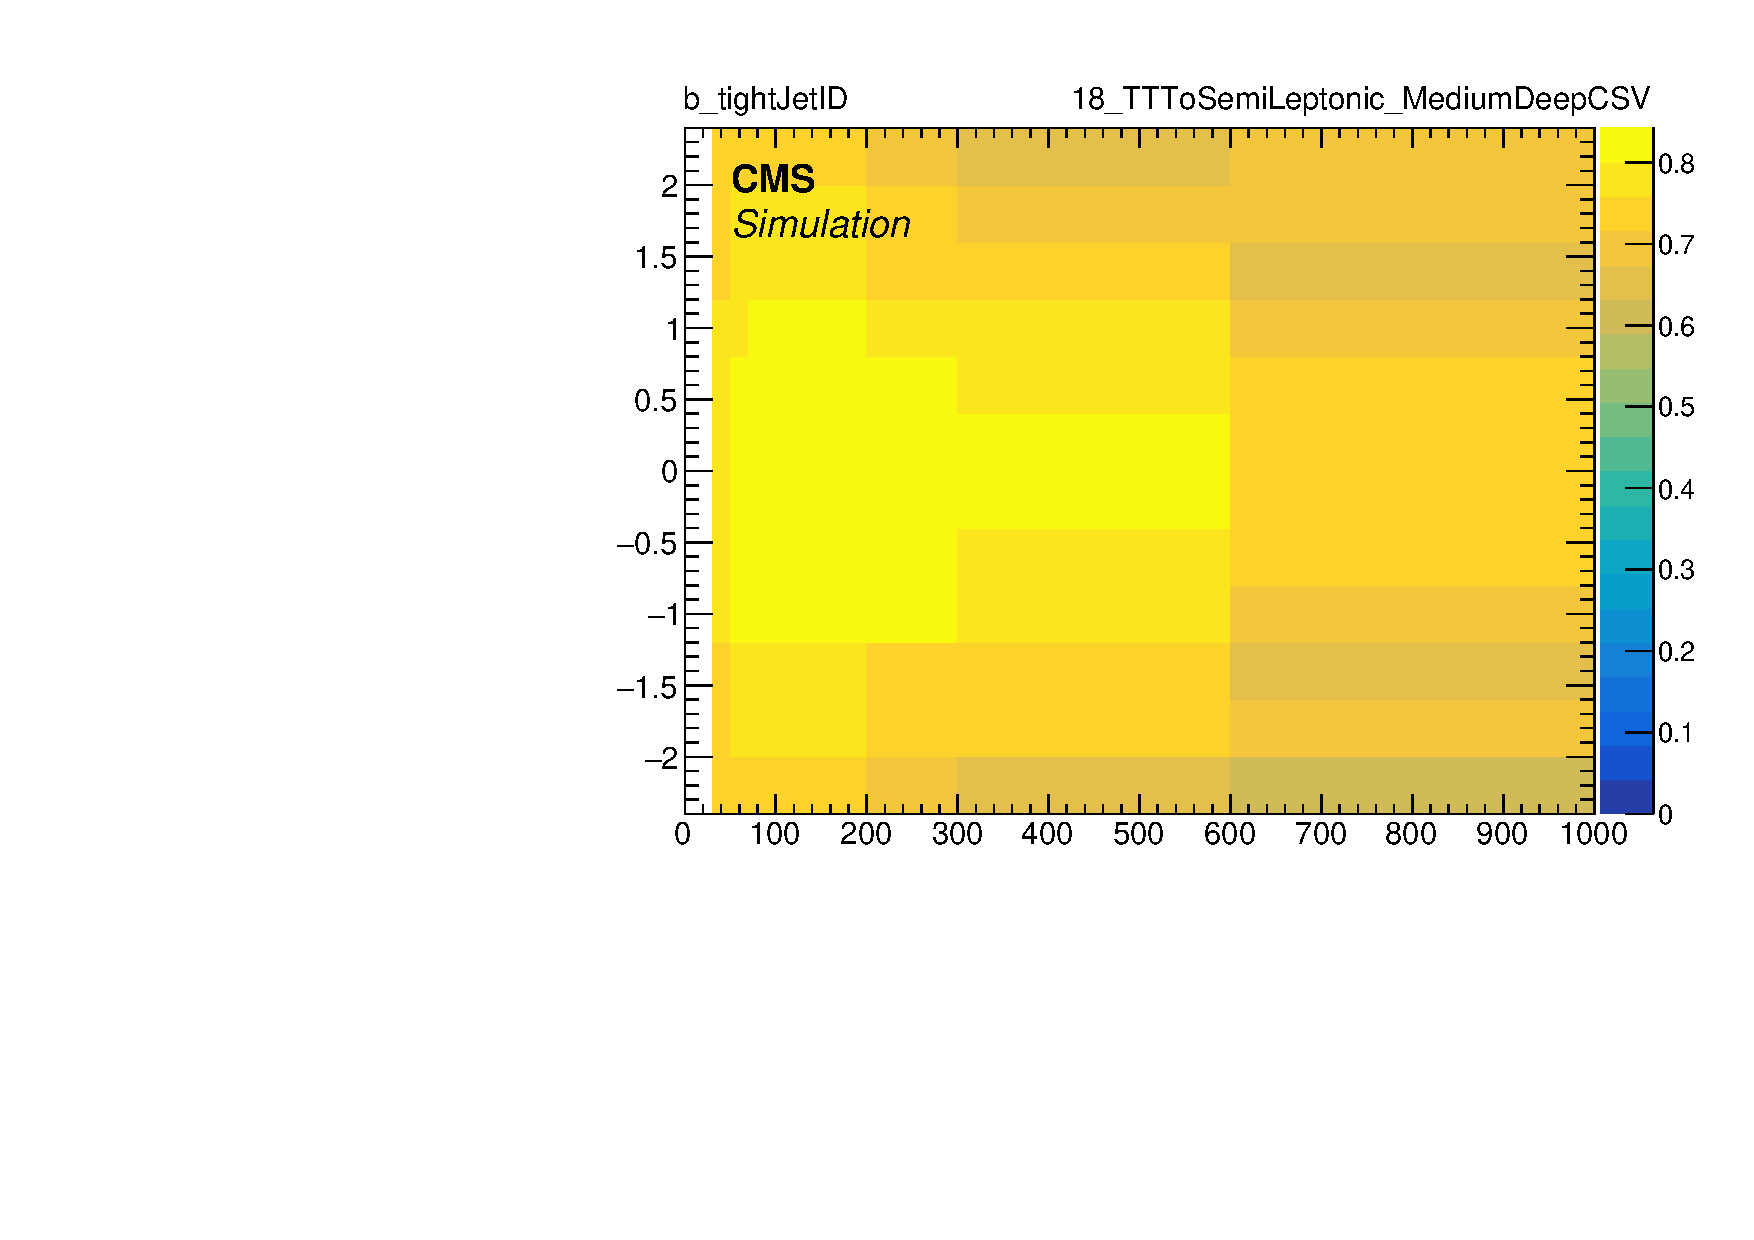
\includegraphics[width=0.4\textwidth]{figure/BtagEffPlot_18_TTToSemiLeptonic_eff2D_b_MediumDeepCSV.pdf}
    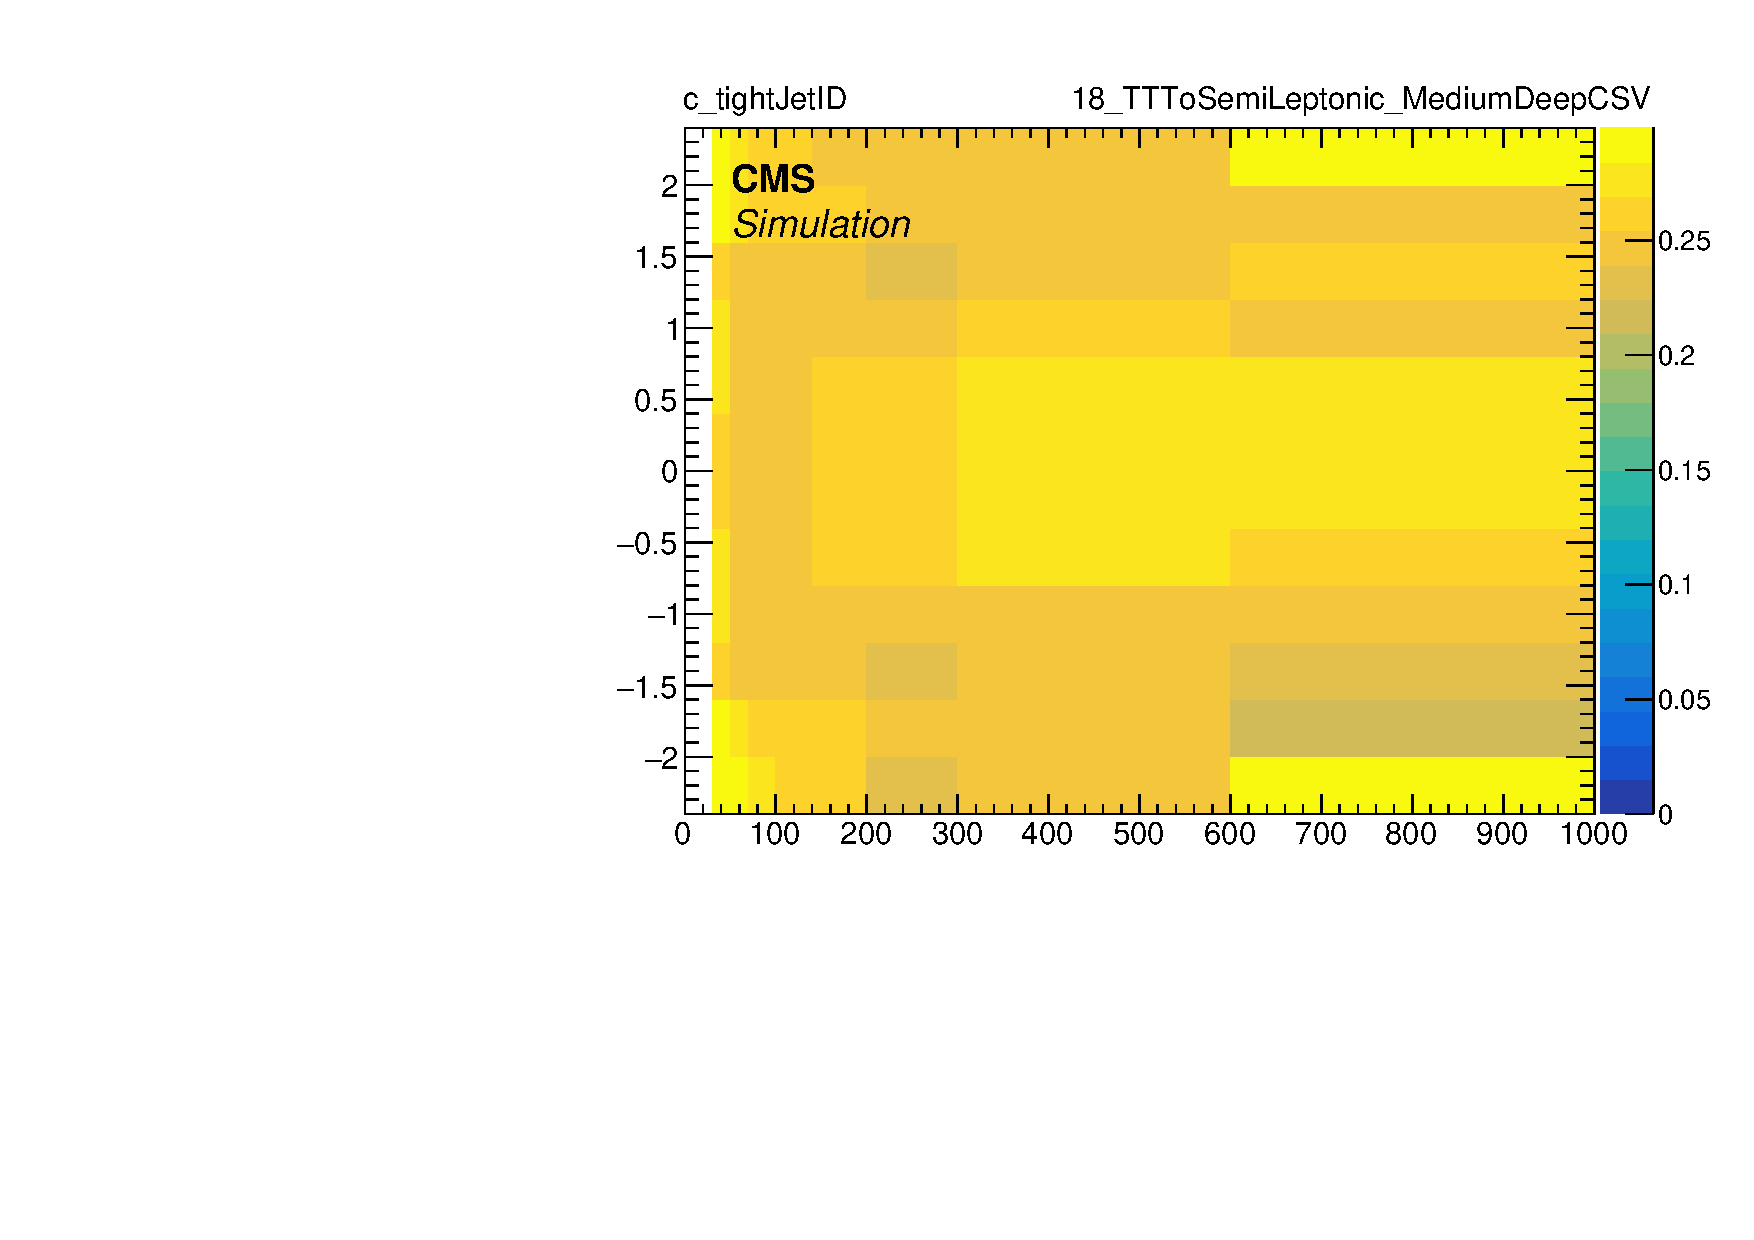
\includegraphics[width=0.4\textwidth]{figure/BtagEffPlot_18_TTToSemiLeptonic_eff2D_c_MediumDeepCSV.pdf}
    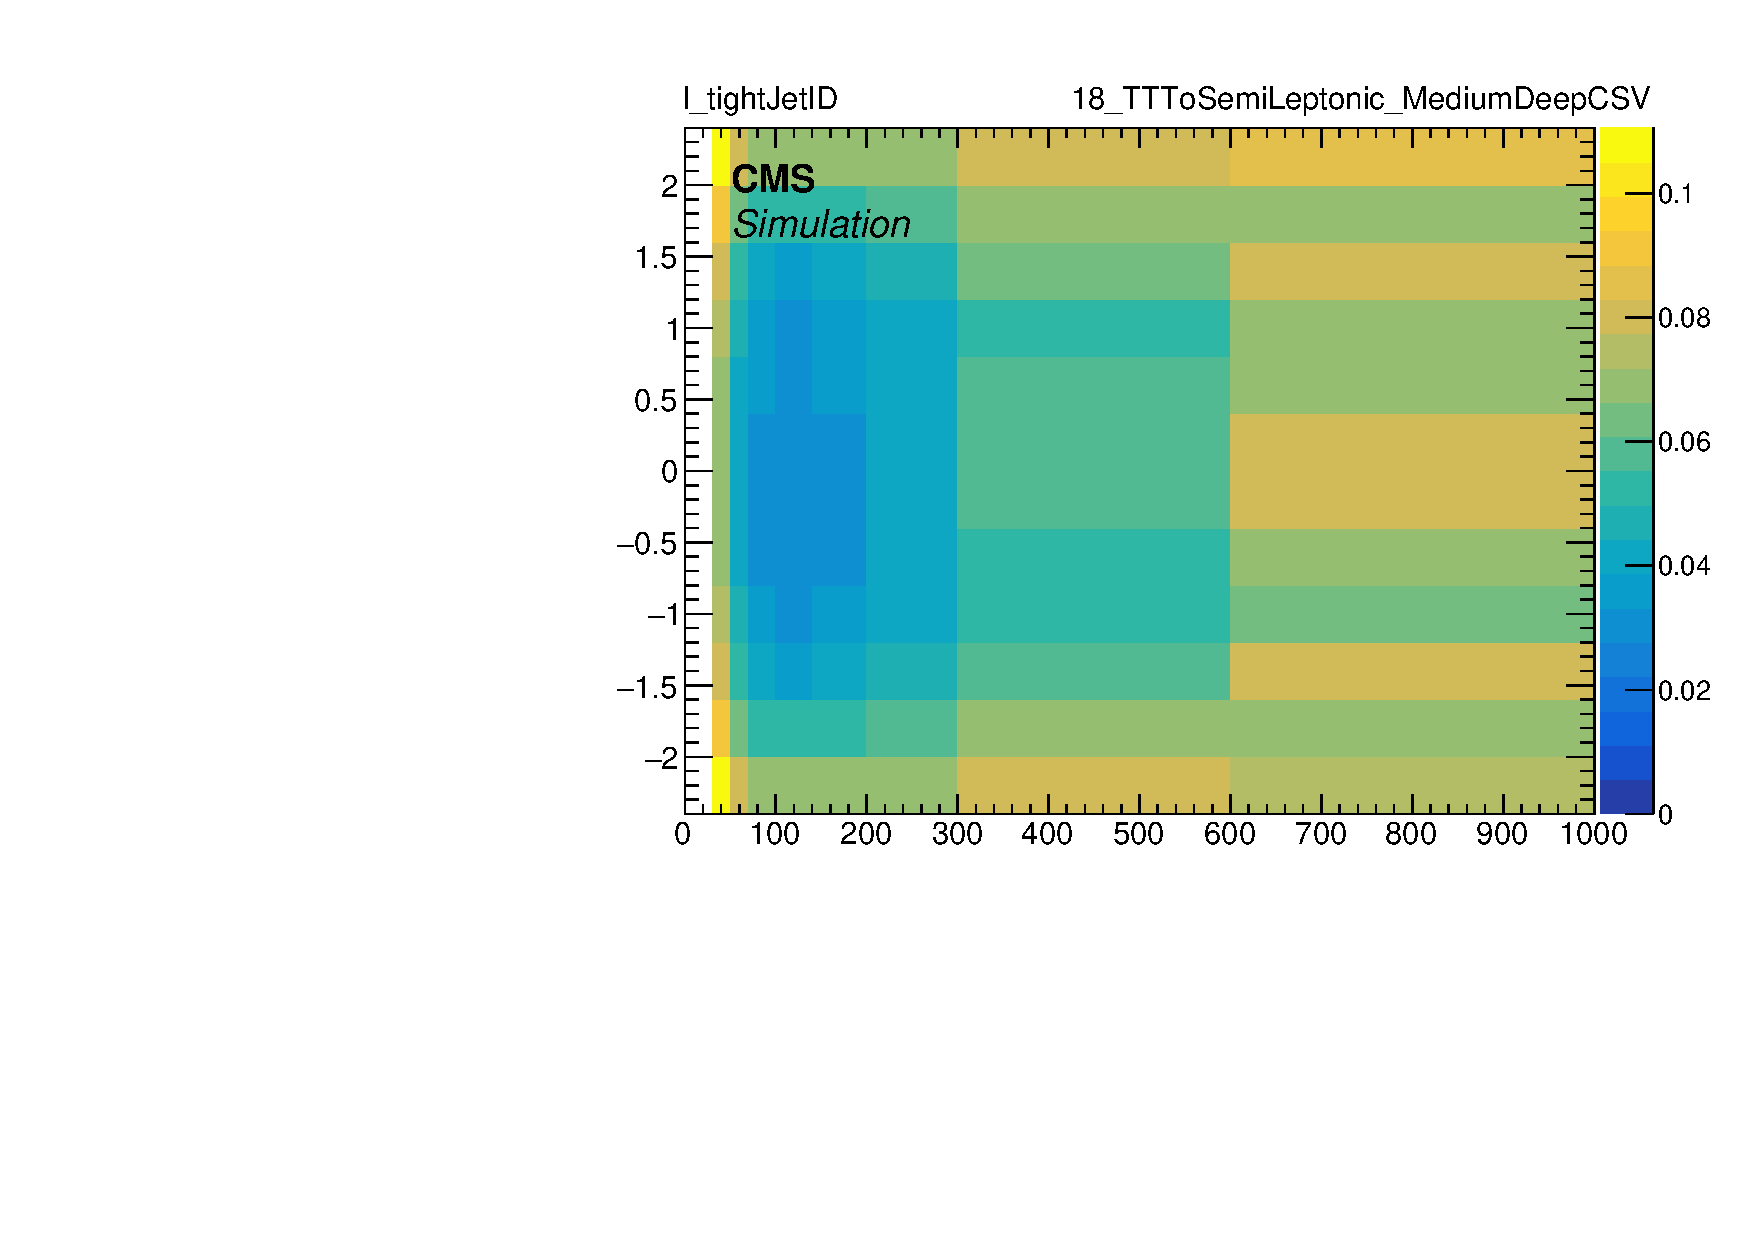
\includegraphics[width=0.4\textwidth]{figure/BtagEffPlot_18_TTToSemiLeptonic_eff2D_l_MediumDeepCSV.pdf}
    \caption[Display of \PQb tagging efficiency of 2018 \ttbar samples.]
    {
        Display of \PQb tagging efficiency of 2018 \ttbar samples for \PQb jet (left), \PQc jet (medium), and light jet (right) as functions of the jet \PT and jet $\eta$.
    }
    \label{fig:reco_beff18}
\end{figure}

\subsection{Pileup re-weighting}
Pileup in data is calculated by comparing the instantaneous luminosity of the proton beams with the total inelastic cross section of pp interaction.
On the other hand, the pileup in simulation is implemented by injecting additional soft interactions other than the main hard processes according to the expected pileup distribution.
However, the simulation typically starts before the actual data taking, and thus the expected pileup distribution might be different from the actual pileup distribution.
Such discrepancies are considered and corrected by re-weighting the simulated events to the actual pileup distribution.

